% !TeX program = pdflatex
% Del circulo cromatico al Tonnetz: la DFT como base propia de la simetria de clases de altura.
% Autor: Carles Marin (con Claude, Anthropic, como asistente de IA).
% Version en espanol de spectral_note.tex (Nota #3 de la serie music-math).
% Build: pdflatex spectral_note_es.tex (dos veces, para refs).

\documentclass[11pt]{article}
\usepackage[T1]{fontenc}
\usepackage[spanish]{babel}
\usepackage{lmodern}
\usepackage{amsmath,amssymb,amsthm,booktabs,graphicx}
\usepackage[hidelinks]{hyperref}
\usepackage{xurl}
\usepackage[table]{xcolor}
\usepackage[margin=1in]{geometry}
\usepackage{microtype}
\usepackage{float}
\usepackage[section]{placeins}
\usepackage{float}
\definecolor{ctA}{HTML}{1B6F8C}
\definecolor{ctB}{HTML}{B5530F}
\setlength{\emergencystretch}{2em}
\newtheorem{theorem}{Teorema}
\newtheorem{proposition}{Proposici\'on}
\newtheorem{remark}{Observaci\'on}
\newcommand{\lean}[1]{\texttt{#1}}
\newcommand{\qlink}[1]{\par\medskip\begin{quote}\itshape\small\color{ctB!88!black}#1\end{quote}\medskip}
\newcommand{\Ztwelve}{\mathbb{Z}_{12}}
\newcommand{\Zn}[1]{\mathbb{Z}_{#1}}
\newcommand{\dft}{\mathcal{F}}
\newcommand{\Ahat}{\hat{A}}
\newcommand{\question}[1]{\smallskip\noindent\textit{#1}\smallskip}

\title{\bf El espectro del Tonnetz es el perfil de balanzas\\ de Fourier de su tr\'iada generadora\\[5pt]
\large\rm un relato verificado por m\'aquina de la simetr\'ia de clases de altura,\\ del c\'irculo crom\'atico al Tonnetz neo-riemanniano}
\author{Carles Mar\'in\thanks{Preparado con la asistencia de un sistema de IA (Claude, Anthropic).
La matem\'atica es cl\'asica; toda afirmaci\'on, alcance y limitaci\'on es responsabilidad del autor, y
es el n\'ucleo de Lean~4 ---no el asistente--- quien certifica las partes formalizadas. El l\'imite de la
contribuci\'on se expone en la Secci\'on~\ref{sec:novelty}.}\\[3pt]
  \normalsize Investigador independiente\\
  \normalsize \texttt{karlesmarin@gmail.com}}
\date{Junio de 2026\\[3pt]\normalsize DOI: \href{https://doi.org/10.5281/zenodo.20862822}{10.5281/zenodo.20862822}
\quad\textbullet\quad \href{https://github.com/karlesmarin/music-math}{github.com/karlesmarin/music-math}}

\begin{document}
\maketitle

\begin{abstract}\noindent
El \textbf{Tonnetz} neo-riemanniano ---el grafo de las $24$ tr\'iadas mayores y menores unidas por los
movimientos parsimoniosos $P,L,R$--- tiene un espectro de adyacencia, y nuestro resultado principal lo
identifica exactamente: \textbf{los autovalores del Tonnetz son $\pm$ las balanzas de Fourier de la \'unica
tr\'iada que lo genera}, el conjunto con signo de autovalores distintos $\pm\{3,\sqrt5,\sqrt3,1,2\cos\frac{\pi}{12},
2\cos\frac{5\pi}{12}\}=\{\pm|\hat{\mathbf 1}_T(k)|\}_{k=0}^{6}$ ($|a_2|=|a_6|=1$ coinciden). La balanza aumentada $\sqrt5=|a_3|$, la
disminuida $\sqrt3=|a_4|$, la de tonos enteros $1=|a_6|$ ---los propios pesos de periodicidad del acorde---
son literalmente las frecuencias de vibraci\'on del grafo (Teorema~\ref{thm:main}). Lo demostramos
construyendo la \'unica herramienta que lo hace inevitable: la DFT es la base propia compartida de la
simetr\'ia de clases de altura. (i)~todo operador invariante por traslaci\'on sobre $\Zn{N}$ (el ciclo
crom\'atico $C_{12}$, todo grafo de Cayley abeliano) queda \textbf{diagonalizado} por los caracteres DFT,
con autovalor el coeficiente de Fourier de su conjunto de conexi\'on (Babai). (ii)~a\~nadir la inversi\'on
hace el grupo $T/I$ $D_{2N}$ \textbf{bloque-diagonal}, emparejando $a_k\leftrightarrow a_{-k}$ en
irreducibles de par conjugado. (iii)~el Tonnetz es el grafo de Cayley del grupo no abeliano $PLR\cong D_{12}$,
y leerlo a trav\'es de (i)--(ii) da la identidad del perfil de balanzas, \emph{completa con multiplicidades}.
Cada paso est\'a verificado por m\'aquina en Lean~4, sin \lean{sorry} y axiom-clean ---incluida la
\textbf{completitud} incondicional del espectro (una base expl\'icita de autovectores; sin Sage, sin
clasificaci\'on de irreps). La f\'ormula espectral en s\'i es est\'andar ---el c\'omputo de Cayley diedral de
Gao--Luo~\cite{GaoLuo}, del que el Tonnetz es la instancia $S=\{P,L,R\}$, y el Laplaciano del Tonnetz lo
estudi\'o Lostanlen. Lo que a\~nadimos es la \emph{lectura} de ese espectro de adyacencia como perfil de
balanzas de la tr\'iada generadora, la identificaci\'on de sus fibras espectrales con la $Z$-relaci\'on
musical (acordes homom\'etricos dan grafos cospectrales ---el viejo criterio de Babai, le\'ido musicalmente)
y la certificaci\'on en Lean. No es matem\'atica nueva ---un relato unificado y certificado.
\end{abstract}

\section{El resultado principal, y la \'unica idea detr\'as}\label{sec:hook}

Un acorde es un conjunto de clases de altura $A\subseteq\Ztwelve$. Codif\'icalo por su indicador $0/1$ y toma
la DFT $\Ahat$; sus coeficientes $a_k=\Ahat(k)$ son las \textbf{balanzas de Fourier} de Lewin y
Quinn~\cite{Quinn} ---$a_1$ mide el agrupamiento crom\'atico, $a_3$ el contenido aumentado, $a_4$ el de
s\'eptima disminuida, $a_5$ el diat\'onico, $a_6$ el de tonos enteros (el diccionario est\'andar, fijado por
qu\'e escala maximiza cada $|a_k|$). Pero los acordes mismos forman tambi\'en un \emph{grafo}: el
\textbf{Tonnetz} neo-riemanniano, cuyos $24$ v\'ertices son las tr\'iadas mayores y menores y cuyas aristas
son los tres movimientos parsimoniosos $P$ (paralelo), $L$ (de sensible), $R$ (relativo), cada uno cambiando
una voz. Esta nota trata de un solo n\'umero asociado a ese grafo ---su espectro de adyacencia--- y la
sorpresa es que no es dato nuevo en absoluto.

\begin{theorem}[Espectro del Tonnetz $=$ perfil de balanzas de la tr\'iada generadora]\label{thm:main}
Sea $A$ el operador de adyacencia del Tonnetz $PLR$ neo-riemanniano sobre las $24$ tr\'iadas mayores/menores,
con tr\'iada generadora $T=\{0,3,7\}$ (clase de conjunto 3-11). Los autovalores de $A$ son exactamente
$\pm|\hat{\mathbf 1}_T(k)|$ para $k=0,\dots,6$ ---el conjunto con signo de valores distintos de las propias balanzas de
Fourier de $T$, $\pm\{3,\sqrt5,\sqrt3,1,2\cos\tfrac{\pi}{12},2\cos\tfrac{5\pi}{12}\}$--- con multiplicidades
dadas por el polinomio caracter\'istico $(x-3)(x+3)(x-1)^3(x+1)^3(x^2-5)^2(x^2-3)^2(x^4-4x^2+1)^2$. Los
autovalores est\'an verificados por m\'aquina en \lean{TonnetzSpectrum.lean}; que sean \emph{todos} ellos
(completitud) en \lean{TonnetzCompleteness.lean}.
\end{theorem}

\question{\textquestiondown Por qu\'e el color arm\'onico de un acorde ---su contenido aumentado, disminuido,
de tonos enteros--- habr\'ia de ser el mismo dato que las frecuencias de vibraci\'on del grafo que ese acorde
genera?}

\noindent Porque ambos los lee \emph{una sola base propia}. Los caracteres DFT diagonalizan simult\'aneamente
todo operador invariante por traslaci\'on; a\~nadir la inversi\'on los pliega en bloques de par conjugado; y
el Tonnetz, siendo el grafo de Cayley del grupo diedral $PLR\cong D_{12}$, se gobierna por exactamente esos
bloques ---as\'i que sus autovalores no pueden ser otra cosa que las balanzas de la tr\'iada generadora. La
nota es esa \'unica idea, construida pelda\~no a pelda\~no (\S\S\ref{sec:setup}--\ref{sec:tonnetz}) hasta el
Teorema~\ref{thm:main}, luego su geometr\'ia (\S\ref{sec:geometry}), su certificaci\'on en Lean
(\S\ref{sec:checked}) y su frontera honesta (\S\ref{sec:novelty}). Donde la Nota~\#1~\cite{Note1} sigui\'o un
\emph{acorde} hacia la teor\'ia de grupos y la Nota~\#2~\cite{Note2} una \emph{pregunta} hacia la fase de
$\Ahat$, esta nota sigue un \emph{espectro} de vuelta a su acorde.

\section{Preliminares: caracteres, circulantes y la base propia DFT}\label{sec:setup}

Fijamos un universo $\Zn{N}$. El \lean{ZMod.dft} de Mathlib (Loeffler~\cite{Loeffler}) se construye sobre el
car\'acter aditivo est\'andar $\mathrm{stdAddChar}\,j=e^{2\pi ij/N}$. El \textbf{$k$-\'esimo car\'acter DFT}
es el vector $\mathrm{dftChar}\,k\,(j)=e^{2\pi i\,jk/N}$. Estos $N$ vectores forman una \textbf{base} de
$\mathbb{C}^{\Zn{N}}$. Una matriz \textbf{circulante} $\mathrm{circulant}\,v$ tiene entrada
$(i,j)\mapsto v(i-j)$ ---un operador invariante por desplazamiento (convoluci\'on); todo operador invariante
por traslaci\'on sobre $\Zn{N}$ es una circulante.

\section{El suelo abeliano: circulantes y grafos de Cayley diagonalizados por la DFT}\label{sec:abelian}

\textbf{La clave de b\'oveda.} Toda circulante se diagonaliza por los caracteres DFT, siendo el autovalor
exactamente el coeficiente de Fourier de su primera columna:
\[
  (\mathrm{circulant}\,v)\,\mathrm{dftChar}\,k \;=\; \hat v(k)\cdot\mathrm{dftChar}\,k
  \qquad(\lean{circulant\_mulVec\_dftChar}).
\]
La prueba es un reindexado m\'as la ley de caracteres; sin an\'alisis. Como los caracteres son base, la DFT
es la base propia diagonalizante \emph{simult\'anea} de todos los operadores invariantes por desplazamiento.

\textbf{El c\'irculo crom\'atico.} La adyacencia de $C_{12}$ es la circulante del indicador de semitono
$\pm1$, as\'i que sus autovalores colapsan al $2\cos(2\pi k/12)$ de manual (\lean{C12\_eigenvalue\_cos}); y
ese $C_{12}$ \emph{es} el grafo de Mathlib,
$\lean{C12\_eq\_adjMatrix}: C_{12}=(\texttt{cycleGraph}\ 12).\mathrm{adjMatrix}\,\mathbb{C}$. La balanza
arm\'onica $a_k$ y el autovalor geom\'etrico $2\cos(2\pi k/12)$ se leen del \emph{mismo} autovector ---la
pregunta de \S\ref{sec:hook}, respondida en el suelo abeliano.

\textbf{Todo grafo de Cayley abeliano.} La clave no es exclusiva de $C_{12}$. Para cualquier conjunto de
conexi\'on $S\subseteq\Zn{N}$, la circulante $\mathrm{cayleyAdj}\,S$ de su indicador se diagonaliza por la
DFT con autovalor la \textbf{suma de caracteres de Babai}~\cite{Babai}
$\sum_{s\in S}\mathrm{stdAddChar}(-(sk))$ (\lean{cayleyAdj\_eigenvalue}), y para $S=-S$ \emph{sim\'etrico}
con $0\notin S$ coincide con la adyacencia de Cayley de Mathlib $\mathrm{circulantGraph}\,S$
(\lean{cayleyAdj\_eq\_adjMatrix}). El c\'irculo crom\'atico es el caso $S=\{1,-1\}$.

\qlink{La DFT diagonaliza todo lo que conmuta con la transposici\'on. Pero la m\'usica tambi\'en
\emph{invierte} ---lee un acorde del rev\'es. ¿Sobrevive la base propia al a\~nadir $I$, o se hace a\~nicos
la diagonal limpia?}

\section{A\~nadir la inversi\'on: la descomposici\'on en bloques diedrales}\label{sec:dihedral}

Hasta aqu\'i s\'olo ha actuado la \emph{traslaci\'on} $T_a$. La \textbf{inversi\'on} $I:x\mapsto-x$ voltea el
c\'irculo crom\'atico, y $T$ con $I$ generan el grupo $T/I$ diedral $D_{2N}$. Directamente sobre los
caracteres,
\[
\begin{aligned}
  I\cdot\mathrm{dftChar}\,k &= \mathrm{dftChar}(-k) && (\lean{inv\_dftChar}),\\[2pt]
  T_a\cdot\mathrm{dftChar}\,k &= \mathrm{stdAddChar}(-(ak))\cdot\mathrm{dftChar}\,k && (\lean{transl\_dftChar}):
\end{aligned}
\]
la traslaci\'on es diagonal; la inversi\'on permuta los caracteres negando la frecuencia. As\'i $D_{2N}$ s\'olo
empareja $k$ con $-k$. Luego el bloque $2$-dimensional $\mathrm{block}\,k=\mathrm{span}\{\mathrm{dftChar}\,k,
\mathrm{dftChar}(-k)\}$ es cerrado bajo inversi\'on y toda traslaci\'on (\lean{block\_dihedral\_invariant})
---la bloque-diagonalizaci\'on de la acci\'on diedral en la base DFT, indexada por los \textbf{pares
conjugados} $\{k,-k\}$. Para $k\neq-k$ el bloque es \textbf{irreducible} (\lean{block\_irreducible}, por
separaci\'on de autovalores): los genuinos irreducibles diedrales $2$-dimensionales, realizados en la base de
Fourier. Por eso el programa ``generativo $\mathbb{C}[D_{2N}]$'' colapsa a la DFT abeliana \emph{cocientada
por inversi\'on}.

\textbf{El tritono, otra vez.} El bloque es $1$-dimensional exactamente cuando $k=-k$, i.e.\ $k\in\{0,N/2\}$:
para $N$ impar s\'olo el DC, pero para \emph{todo} $N=2m$ par tambi\'en el \textbf{tritono} $N/2$, fijo por
inversi\'on en todo universo par (\lean{tritone\_selfPaired}). El n\'umero de bloques $1$-dimensionales es
$\gcd(2,N)$. El tritono es la \'unica frecuencia no nula auto-conjugada ---el mismo $T_6$ que centra la
autodualidad 6-30 de la Nota~\#1 y la paridad del vector \'indice de la Nota~\#2. Todo \S\ref{sec:dihedral}
vale para \emph{todo} $N$.

\textbf{Cualquier temperamento igual, gratis.} Como todo teorema anterior se enuncia sobre un $\Zn{N}$
arbitrario, la descomposici\'on en bloques se instancia en \emph{cualquier} temperamento igual sin prueba
adicional ---un dividendo concreto de formalizar sobre un par\'ametro en vez de a mano. En los sistemas
microtonales 19-, 31- y 53-TET (todos impares) no hay tritono alguno: la \'unica frecuencia auto-pareada
es el DC, $\gcd(2,N)=1$, luego un solo bloque $1$-dimensional y $(N-1)/2$ bloques $2$-dimensionales
irreducibles (\lean{block\_irreducible} es gen\'erico). En un temperamento par como 24-TET (cuartos de
tono) el tritono reaparece en $N/2=12$, dando dos bloques $1$-dim. El asistente de pruebas confirma cada
caso con una aplicaci\'on del censo gen\'erico ---p.\,ej.\ \lean{(\{k : ZMod 19 | k = -k\}).ncard = 1} y
\lean{tritone\_selfPaired 12} para 24-TET---, todo verificado por m\'aquina en \lean{InversionDFT.lean}: la
familia entera surge del \'unico teorema universal en $N$.

\textbf{La unificaci\'on con la Nota~\#2 (verificada por m\'aquina).} Para un indicador real $0/1$ la DFT es
hermitiana, $\Ahat(-t)=\overline{\Ahat(t)}$ (\lean{Ahat\_neg}), as\'i que el espectro de potencia es
\textbf{constante en cada par conjugado}, $|\Ahat|^2(-t)=|\Ahat|^2(t)$ (\lean{powerSpec\_neg}) ---desciende
al cociente de inversi\'on $\Zn{N}/(t\sim-t)$, el propio conjunto de pares conjugados. El vector de
intervalos es su pliegue sobre esos pares,
$\mathrm{IVraw}(A,k)=\dft^{-1}(|\Ahat|^2)(k)+\dft^{-1}(|\Ahat|^2)(-k)$ para $1\le k\le5$
(\lean{IVraw\_eq\_powerSpec\_conjPair}). As\'i el suelo ciego a la fase de la Nota~\#2 (homometr\'ia $=$
$|\Ahat|^2$ igual) y los bloques diedrales de la Nota~\#3 son \emph{el mismo objeto de par conjugado}. Las
dos mitades son cl\'asicas ---la redundancia hermitiana~\cite{Amiot,MGAAA} y los irreducibles diedrales
indexados por $\{k,-k\}$~\cite{CFS}; lo que observamos es que los dos indexados conocidos son un solo objeto.

\qlink{Los bloques $\pm k$ son teor\'ia de representaciones abstracta ---contabilidad de irreducibles. ¿Hay
un objeto musical \emph{concreto}, un grafo que se pueda dibujar en el Tonnetz, cuyo espectro de adyacencia
\emph{sea} sin m\'as esa estructura de bloques hecha sonido?}

\section{Teorema principal: el espectro del Tonnetz es el perfil de balanzas de la tr\'iada}\label{sec:tonnetz}

El \'ultimo pelda\~no abandona el mundo abeliano y aterriza en el Teorema~\ref{thm:main}. El \textbf{grupo
$PLR$} neo-riemanniano ---generado por las
involuciones \emph{Parallel}, \emph{Leading-tone} y \emph{Relative} sobre las 24 tr\'iadas mayores/menores---
es \'el mismo $\cong D_{12}$ (Crans--Fiore--Satyendra~\cite{CFS}). Su grafo de Cayley $\Gamma$ es el
\textbf{Tonnetz}, el toro de tela met\'alica de Douthett--Steinbach~\cite{DS}: $24$ v\'ertices, $3$-regular.
El operador de adyacencia $A$ es sim\'etrico y $3$-regular, con dos autovalores racionales: $\mathbf{+3}$ (el
vector de unos, irrep trivial) y $\mathbf{-3}$ (el vector \emph{signo} mayor/menor ---toda arista del
Tonnetz cruza mayor$\leftrightarrow$menor, $\Gamma$ es \textbf{bipartito en la cualidad}). El resto se
gobierna por los irreducibles diedrales ---y aqu\'i un hecho \emph{general} hace el trabajo, del que el
Tonnetz es una instancia.

\begin{proposition}[Espectro de Cayley diedral; Gao--Luo~\cite{GaoLuo}, cf.\ el survey de Liu~\cite{LiuSurvey}]\label{prop:dihedral}
Sea $S\subseteq\Zn{N}$ y form\'ese el grafo de Cayley de $D_{2N}$ sobre el conjunto de conexi\'on de
\emph{reflexiones} $\{s\,r^{c}:c\in S\}$. Su espectro de adyacencia es
\[
  \pm\bigl\{\,|\hat{\mathbf 1}_S(k)|:k=0,1,\dots,\lfloor N/2\rfloor\,\bigr\},\qquad
  \hat{\mathbf 1}_S(k)=\sum_{c\in S}\omega^{kc},\quad \omega=e^{2\pi i/N},
\]
el $\pm$ por bipartici\'on (toda arista de reflexi\'on intercambia rotaciones y reflexiones).
\end{proposition}
\noindent\textit{Prueba (conceptual).}~En la irrep $2$-dimensional $\rho_k$
($r\mapsto\mathrm{diag}(\omega^{k},\omega^{-k})$, $s\mapsto\left(\begin{smallmatrix}0&1\\1&0\end{smallmatrix}\right)$)
el operador $\sum_{c\in S}\rho_k(s\,r^{c})$ es el bloque antidiagonal
$\left(\begin{smallmatrix}0&\hat{\mathbf 1}_S(k)\\[1pt]\overline{\hat{\mathbf 1}_S(k)}&0\end{smallmatrix}\right)$,
con autovalores $\pm|\hat{\mathbf 1}_S(k)|$; las irreps $1$-dimensionales dan $\pm|\hat{\mathbf 1}_S(0)|$ y
$\pm|\hat{\mathbf 1}_S(N/2)|$. El espectro de Cayley es la uni\'on sobre irreps (Babai~\cite{Babai}).\hfill$\square$

\smallskip\noindent Es est\'andar; lo registramos s\'olo para situar la m\'usica. \textbf{El
Teorema~\ref{thm:main} es el caso $N=12$, $S=\{P,L,R\}$.} El conjunto de conexi\'on $PLR$, en coordenadas de
desplazamiento de fundamental, es una transposici\'on de la tr\'iada generadora $T=\{0,3,7\}$, as\'i
$\hat{\mathbf 1}_S(k)=|a_k(T)|$ y el espectro es el propio multiconjunto de balanzas de la tr\'iada
\[
  \pm\{\,3,\ \sqrt5,\ 2\cos(\tfrac{\pi}{12}),\ \sqrt3,\ 1,\ 2\cos(\tfrac{5\pi}{12})\,\},
\]
polinomio caracter\'istico $(x-3)(x+3)(x-1)^3(x+1)^3(x^2-5)^2(x^2-3)^2(x^4-4x^2+1)^2$, con el \textbf{dorado}
$\sqrt5=|1+2i|=|a_3|$ la balanza aumentada. La raz\'on conceptual de que el Tonnetz suene como su tr\'iada es
la Proposici\'on~\ref{prop:dihedral}: \emph{un acorde es el conjunto de conexi\'on de su grafo}.

\textbf{Homometr\'ia $\Rightarrow$ cospectral (una entrada de diccionario).} Por la
Proposici\'on~\ref{prop:dihedral} el espectro depende de $S$ solo a trav\'es de
$\{|\hat{\mathbf 1}_S(k)|\}$ ---el vector de intervalos de $S$. As\'i, dos conjuntos de clases de altura
\textbf{homom\'etricos} ($Z$-relacionados: mismo vector de intervalos, mismo $|\hat{\mathbf 1}|$) generan
grafos de Cayley diedrales \emph{cospectrales}. La implicaci\'on es vieja ---es el criterio de cospectralidad
por multiconjunto de diferencias de Babai~(\cite{Babai}, Cor.~4.2), usado para fabricar diedrales
cospectrales por Abdollahi--Janbaz--Ghahramani~\cite{Abdollahi}; lo nuevo aqu\'i es solo la
\emph{identificaci\'on} de ese multiconjunto de diferencias con el vector de intervalos musical, ligando la
fibra espectral a la $Z$-relaci\'on de la Nota~\#2~\cite{Note2}. Por ejemplo los tetracordes todo-intervalo
$4$-Z15~$\{0,1,4,6\}$ y $4$-Z29~$\{0,1,3,7\}$ son homom\'etricos pero no $T/I$-relacionados ---luego
cospectrales pero no isomorfos.

\textbf{Verificado por m\'aquina.} Cada autovalor se certifica en Lean por un autovector expl\'icito
$Au=\lambda u$ (\lean{A\_mulVec\_golden}, \lean{A\_mulVec\_j4/j2/j1/j5}), la mitad negativa gratis por el
volteo de cualidad (\lean{bipartite\_neg\_eigen}); y la \emph{completitud} ---que estos $24$ sean
\emph{todos}--- tambi\'en (\lean{tonnetz\_spectrum\_complete\_unconditional}): los autovectores forman una
\emph{base} expl\'icita de $\mathbb{C}^{\mathrm{Triad}}$, as\'i que el espectro es exactamente el
multiconjunto $\{\pm|\hat{\mathbf 1}_T(k)|\}_{k=0}^{11}$ ---una diagonalizaci\'on completa, \emph{sin} Sage y
\emph{sin} clasificaci\'on en irreps de $D_{12}$ (que Mathlib no tiene). \emph{Evaluar} ese multiconjunto a
las seis formas cerradas nombradas con multiplicidades $1,2,2,3,2,2$ ---el polinomio caracter\'istico
factorizado del Teorema~\ref{thm:main}--- es el testigo exacto de Sage (\lean{tonnetz\_cayley\_spectrum.py}):
Lean certifica la base, Sage los valores nombrados.

\textbf{La lectura musical.} Cada autovalor mide ahora una periodicidad arm\'onica de la tr\'iada generadora
---$\sqrt5=|a_3|$ \textbf{aumentado} (la mayor balanza no
trivial), $\sqrt3=|a_4|$ \textbf{s\'eptima disminuida}, $2\cos(\tfrac{\pi}{12})=|a_5|$ \textbf{diat\'onico},
$2\cos(\tfrac{5\pi}{12})=|a_1|$ \textbf{crom\'atico}, $1=|a_6|$ \textbf{tonos enteros}, $\pm3=|a_0|$
cardinalidad. (Las etiquetas son el diccionario est\'andar Quinn--Amiot, fijado por qu\'e escala maximiza
cada $|a_k|$: tr\'iada aumentada $\to a_3$, s\'eptima disminuida $\to a_4$, escala de tonos enteros $\to
a_6$.) Lostanlen~\cite{Lostanlen} diagonaliz\'o el \emph{Laplaciano} $L=D-A$ del mismo grafo (autovalores
$3-\lambda$, no los de adyacencia) y us\'o sus autovectores como filtros wavelet, sin nombrar nunca los
autovalores ni conectarlos con las balanzas; leer el espectro de adyacencia como el perfil de balanzas de la
tr\'iada parece no estar enunciado.

\qlink{As\'i que el espectro son seis n\'umeros,
$\pm\{3,\sqrt5,\sqrt3,1,2\cos\tfrac{\pi}{12},2\cos\tfrac{5\pi}{12}\}$ ---una lista. Pero una lista esconde
una forma. ¿Qu\'e \emph{aspecto} tiene en realidad la estructura propia cuando dejamos que las rotaciones
giren?}

\section{La geometr\'ia de la estructura espectral}\label{sec:geometry}

Toda la escalera tiene una sola cara geom\'etrica: \textbf{la base de Fourier es un sistema de rotaciones}
(scripts en \lean{viz/}).

\textbf{La transposici\'on es un tren de engranajes} (Figura~\ref{fig:gears}). La transposici\'on multiplica
$a_k$ por $e^{-2\pi ikt/12}$, as\'i que $a_k$ \textbf{gira a velocidad $k$}, visitando $12/\gcd(k,12)$
posiciones antes de repetir; todos los engranajes se re-sincronizan en la octava $t=12$. El DC $a_0$ tiene
velocidad $0$ ---no se mueve (la cardinalidad); el tritono $a_6$ es real, s\'olo cambia de signo; cada par
conjugado es un engranaje y su espejo, contrarrotando a $\pm k$. Engranan en un solo mecanismo cerrado
precisamente porque las velocidades son \textbf{enteras} (conmensurables $\Rightarrow$ peri\'odicas); en una
afinaci\'on irracional el mismo flujo ser\'ia erg\'odico. El radio de cada engranaje es $|a_k|$ ---la balanza
de la tr\'iada, i.e.\ el autovalor del Tonnetz de \S\ref{sec:tonnetz}.

\begin{figure}[tbp]\centering
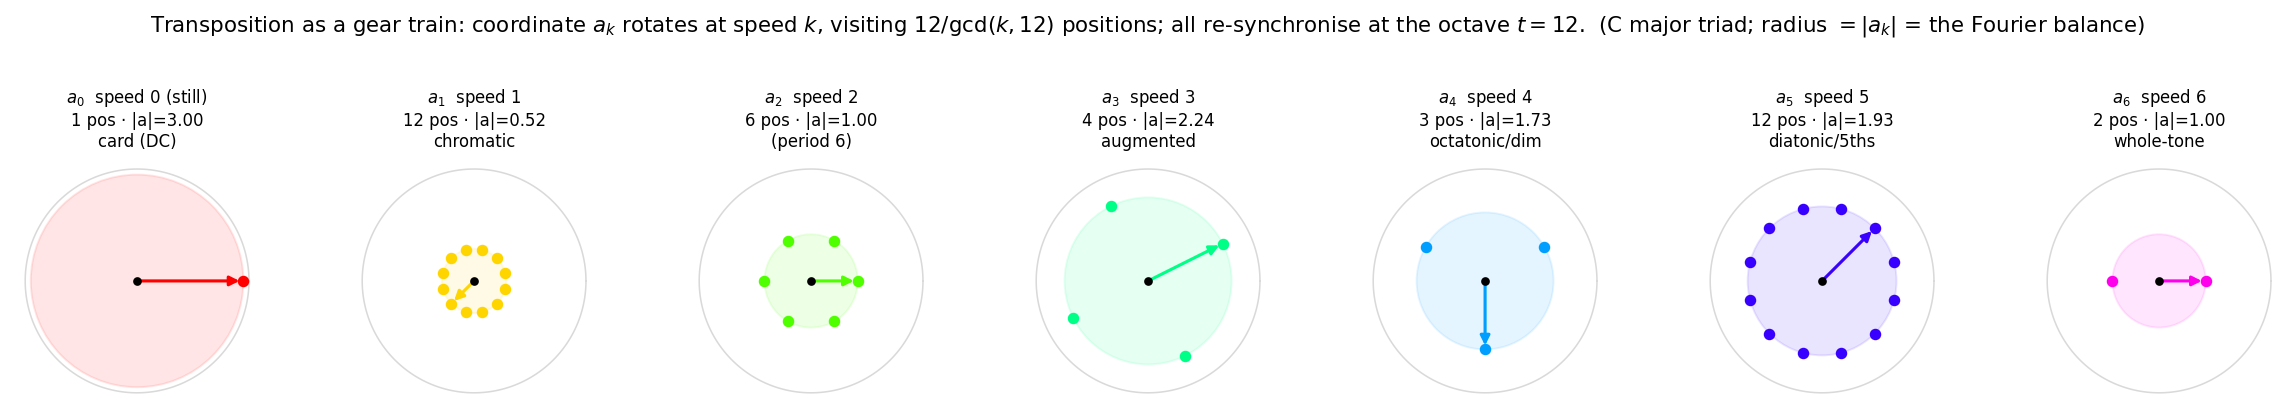
\includegraphics[width=0.74\linewidth]{figs/fig_gears.png}
\caption{La transposici\'on como tren de engranajes: $a_k$ gira a velocidad $k$, visitando $12/\gcd(k,12)$
posiciones; todos se re-sincronizan en la octava. Radio $=|a_k|$, la balanza de Fourier ($a_0$ quieto; $a_3$
aumentado $=\sqrt5$; $a_4$ disminuido $=\sqrt3$; $a_6$ tonos enteros).}
\label{fig:gears}
\end{figure}

\textbf{La inversi\'on pliega la base sobre un toro} (Figura~\ref{fig:crttorus}). El Teorema Chino del Resto
$\Ztwelve\cong\Zn{3}\times\Zn{4}$ ($j\mapsto(j\bmod3,\,j\bmod4)$) parte el universo en dos c\'irculos factor
---el eje \textbf{aumentado} $\langle4\rangle=\{0,4,8\}$ (el factor $\Zn3$) y el eje \textbf{disminuido}
$\langle3\rangle=\{0,3,6,9\}$ (el factor $\Zn4$)--- y un semitono crom\'atico es el paso diagonal. En el lado
dual la partici\'on es exacta, con un peque\~no pero real intercambio de \'indices que conviene precisar.

\begin{proposition}[Coordenadas CRT de los caracteres]\label{prop:crt}
Bajo $\Ztwelve\cong\Zn3\times\Zn4$, un car\'acter $\chi_k$ factoriza por la proyecci\'on a $\Zn3$ sii
$k\in\{0,4,8\}$, y por la proyecci\'on a $\Zn4$ sii $k\in\{0,3,6,9\}$. Por tanto $\chi_4$ genera el eje
aumentado ($\Zn3$) y $\chi_3$ genera el eje disminuido ($\Zn4$), con el tritono $\chi_6$ el elemento de orden
$2$ de la parte $\Zn4$.
\end{proposition}
\noindent\textit{Prueba.}~$\chi_k$ factoriza por $\pi_3:\Ztwelve\to\Zn3$ sii es trivial en
$\ker\pi_3=\{0,3,6,9\}$, i.e.\ $\chi_k(3)=e^{\pi i k/2}=1$, i.e.\ $4\mid k$; sim\'etricamente por $\pi_4$ sii
$\chi_k(4)=e^{2\pi i k/3}=1$, i.e.\ $3\mid k$.\hfill$\square$

\smallskip\noindent El intercambio es la clave: la tr\'iada aumentada \emph{maximiza} $|a_3|$ porque $\chi_3$
es \emph{constante} en ella (factoriza por el cociente $\Zn4$), mientras que el car\'acter que \emph{resuelve}
el eje aumentado es $\chi_4$. As\'i ``qu\'e escala satura $a_k$'' y ``qu\'e $\chi_k$ coordina el factor'' se
leen con los \'indices $3\leftrightarrow4$ cambiados ---dos caras duales de una sola partici\'on CRT.
\emph{Dentro} de un c\'irculo factor los puntos est\'an bloqueados; la diagonal \emph{acopla} los dos
factores en el \'unico reloj crom\'atico ---el mismo factor-vs-diagonal que los bloques de par conjugado de
\S\ref{sec:dihedral} expresan como contrarrotaci\'on vs impulso com\'un.

\begin{figure}[H]\centering
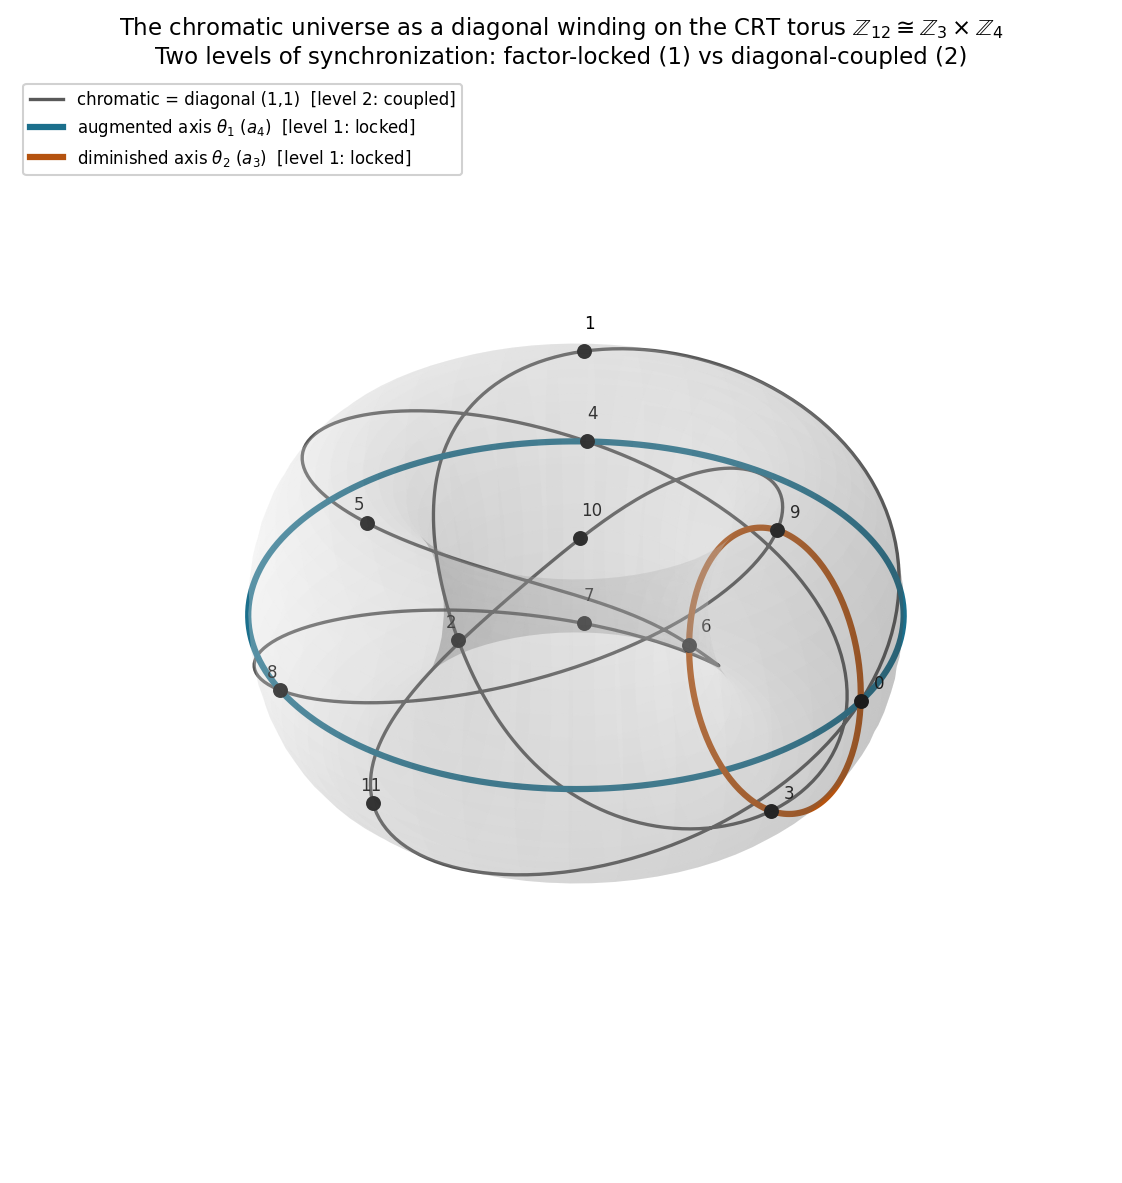
\includegraphics[width=0.62\linewidth]{figs/fig_crttorus.png}
\caption{$\Ztwelve\cong\Zn{3}\times\Zn{4}$ como enrollado diagonal en el toro CRT: los c\'irculos factor son
los ejes aumentado ($\Zn3$, resuelto por $\chi_4$) y disminuido ($\Zn4$, resuelto por $\chi_3$)
(Prop.~\ref{prop:crt}); el crom\'atico es la diagonal. Dos niveles de sincronizaci\'on: factor-bloqueado y
diagonal-acoplado.}
\label{fig:crttorus}
\end{figure}

\textbf{Por qu\'e el tritono siembra cada mitad.} Antes de la geometr\'ia, el \'algebra que la impulsa.
Modela el c\'irculo de clases de altura como $S^1=\mathbb{R}/\mathbb{Z}$; la temperaci\'on igual de $2^n$
tonos es el subgrupo $\mu_{2^n}\cong\Zn{2^n}$ de ra\'ices $2^n$-\'esimas de la unidad, y la bisecci\'on de
octava las anida $\Zn{2}\subset\Zn{4}\subset\Zn{8}\subset\cdots$. El mapa que enlaza un nivel con el
siguiente es la \textbf{duplicaci\'on} $\delta:z\mapsto z^2$ (en \'angulos $\theta\mapsto2\theta$), el
plegado de octava $2$-a-$1$ del c\'irculo. Es exactamente $2$-a-$1$: la fibra de $\delta$ sobre el unísono
$z=1$ es $\{z:z^2=1\}=\{+1,-1\}$, y $-1=e^{\pi i}$ es el \textbf{tritono}, el \'unico elemento de orden $2$
de $S^1$ (\lean{tritone\_selfPaired}, en todo nivel par). As\'i la pregunta binaria de cada etapa ---``¿qu\'e
ra\'iz cuadrada del unísono?''--- es justo ``¿unísono o tritono?'': el tritono es el elemento no trivial de
toda fibra de enlace.

\textbf{La torre di\'adica: un teorema, y una analog\'ia honesta} (Figura~\ref{fig:solenoid}). Iterando la
fibra, los n\'ucleos $\ker\delta^{\,n}=\mu_{2^n}\cong\Zn{2^n}$ forman un sistema proyectivo genuino bajo
duplicaci\'on, y su l\'imite inverso es un \emph{teorema}, no una met\'afora:
$\varprojlim\!\big(\cdots\to\Zn{2^{n+1}}\to\Zn{2^n}\big)\cong\mathbb{Z}_2$, los enteros $2$-\'adicos ---la
fibra de Cantor del solenoide de Smale--Williams $\mathbb{S}_2=\varprojlim(S^1\xleftarrow{\,\delta\,}S^1
\cdots)$, con el tritono el elemento de orden $2$ en cada etapa finita y ninguno sobreviviendo al l\'imite
libre de torsi\'on (geom\'etricamente, $\delta$ enrolla el tubo del toro s\'olido dos veces alrededor de su
n\'ucleo; la intersecci\'on anidada $\bigcap_n\delta^{\,n}(\text{tubo})$ es el atractor). \textbf{Lo que
\emph{no} afirmamos} es un teorema que identifique la descomposici\'on en bloques de \S\ref{sec:dihedral}
---que vive en un $N$ fijo--- \emph{con} este solenoide. La ruta tentadora falla limpiamente, y registramos
el negativo: los caracteres auto-pareados $\chi_{2^{n-1}}$ son \emph{todos} el mismo car\'acter signo
$(-1)^j$, as\'i que la torre ingenua de subespacios auto-pareados $V_n=\langle\chi_0,\chi_{2^{n-1}}\rangle$
es constante y $\varprojlim V_n$ es solo $\mathbb{C}^2$, no $\mathbb{S}_2$. Por tanto conservamos el
solenoide como una \emph{imagen} de la torre de rejillas di\'adicas, no como corolario del teorema de
bloques; el puente preciso ---un sistema proyectivo construido con los datos de bloque y convergente a
$\mathbb{S}_2$--- lo marcamos como \textbf{abierto} (\S\ref{sec:novelty}). \emph{El solenoide y lo
$2$-\'adico en m\'usica son cl\'asicos (Pitk\"anen~\cite{Pitkanen}; Fokker~\cite{Fokker}; el toro
$\Zn{4}$/disminuido est\'a en Yust~\cite{YustGT}); a\~nadimos solo la lectura del tritono v\'ia la fibra de
duplicaci\'on y el negativo expl\'icito de arriba.}

\begin{figure}[H]\centering
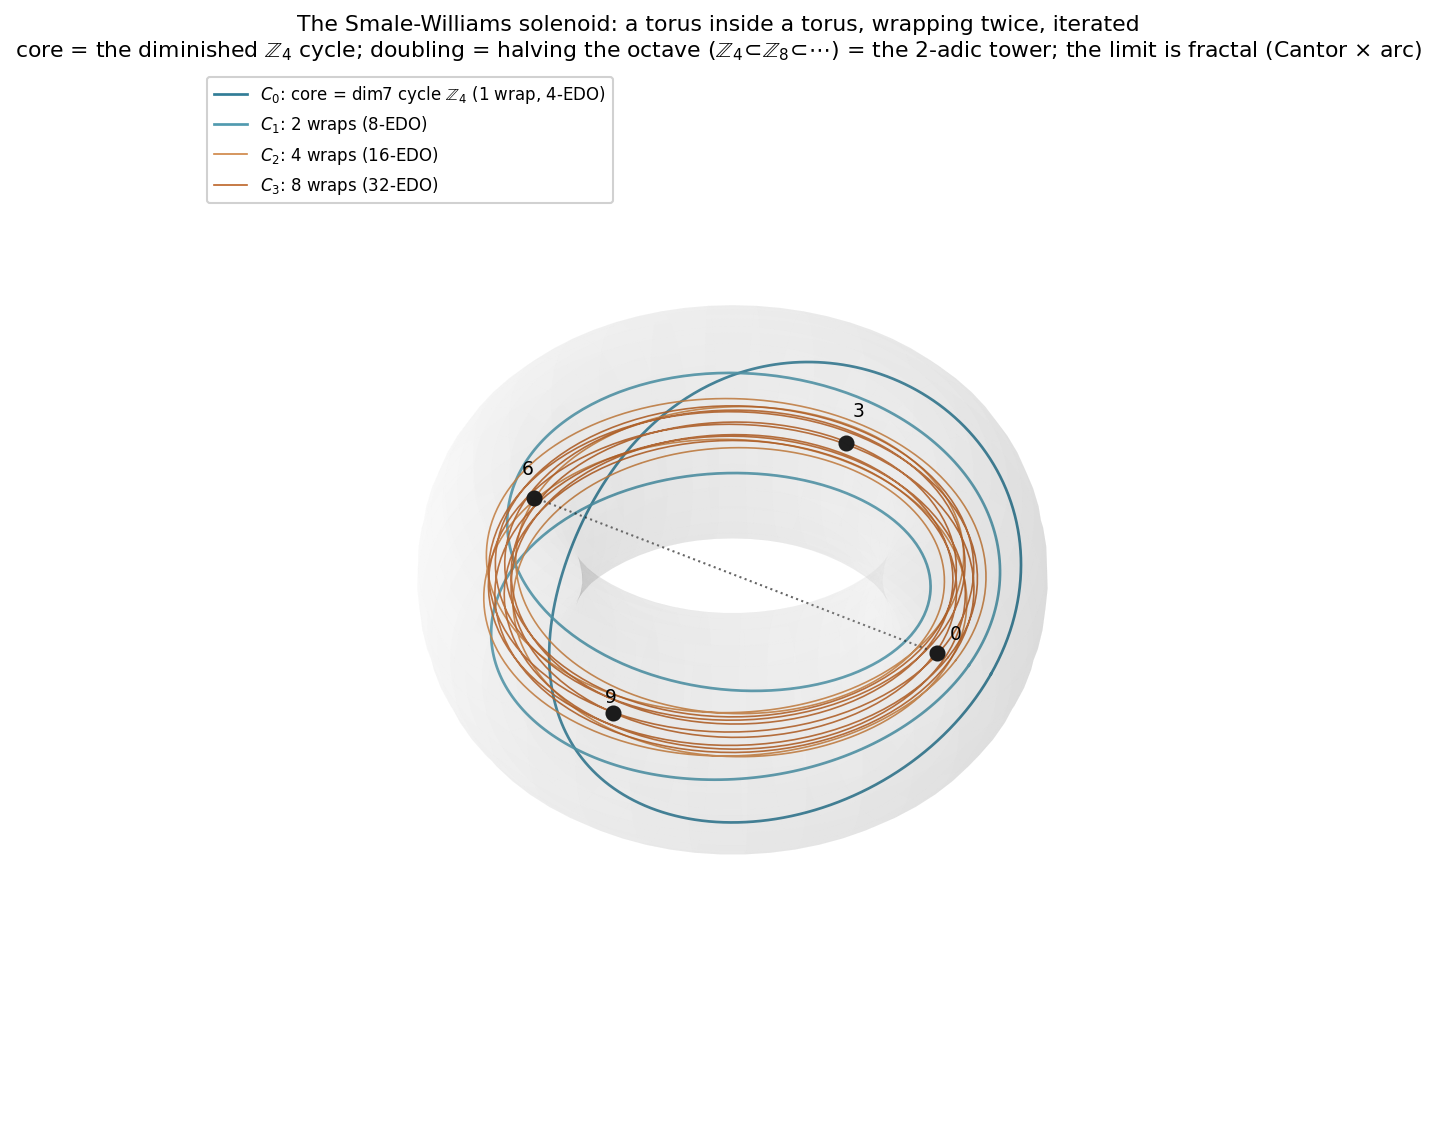
\includegraphics[width=0.66\linewidth]{figs/fig_solenoid.png}
\caption{El solenoide de Smale--Williams: un toro enrollado dos veces dentro de un toro, iterado. La
duplicaci\'on $\delta:z\mapsto z^2$ es $2$-a-$1$, con fibra $\{$unísono$,$ tritono$\}$ sobre el unísono; el
l\'imite inverso $\varprojlim(S^1\xleftarrow{\delta}S^1\cdots)$ tiene fibra de Cantor ($\mathbb{Z}_2$)
construida con esas elecciones binarias. Lo usamos como imagen de la torre de rejillas di\'adicas, no como
corolario del teorema de bloques (ver texto).}
\label{fig:solenoid}
\end{figure}

\qlink{Cada paso hasta aqu\'i ha \emph{afirmado} un teorema. Pero una afirmaci\'on no es una prueba, y un
diagrama no es un certificado. ¿Cu\'ales de ellos verifica de verdad un n\'ucleo de pruebas ---y a qu\'e
coste axiom\'atico?}

\section{Qu\'e est\'a verificado por m\'aquina}\label{sec:checked}

La escalera espectral ---ahora incluyendo la completitud--- la certifica el n\'ucleo de Lean~4 en cinco
archivos sin \lean{sorry}, cada uno con una auditor\'ia de axiomas (\lean{\#print axioms}) que devuelve a lo
sumo \lean{[propext, Classical.choice, Quot.sound]} sin \lean{sorryAx}. Verificado recompilando cada uno
desde cero en el entorno r\'apido godsil (EXIT~0).

\begin{table}[!ht]
\centering\footnotesize
\setlength{\tabcolsep}{4pt}
\rowcolors{2}{ctA!7}{white}
\begin{tabular}{@{}p{0.29\textwidth} p{0.195\textwidth} p{0.425\textwidth}@{}}
\toprule
\rowcolor{ctA!22}
\textbf{Teorema} & \textbf{Archivo} & \textbf{Enunciado}\\
\midrule
\lean{circulant\_mulVec\_dftChar} & \lean{CycleGraphSpectrum} & Toda circulante diagonalizada por la DFT; autovalor $=\hat v(k)$ (clave).\\
\lean{C12\_eigenvalue\_cos} & \lean{CycleGraphSpectrum} & El espectro de $C_{12}$ es $2\cos(2\pi k/12)$.\\
\lean{C12\_eq\_adjMatrix} & \lean{CycleGraphSpectrum} & $C_{12}$ es la adyacencia de \texttt{cycleGraph 12} de Mathlib.\\
\lean{cayleyAdj\_eigenvalue} & \lean{CycleGraphSpectrum} & Espectro de Cayley abeliano $=\sum_{s\in S}\mathrm{stdAddChar}(-(sk))$ (Babai).\\
\lean{inv\_dftChar} / \lean{transl\_dftChar} & \lean{InversionDFT} & La inversi\'on intercambia $k\leftrightarrow-k$; la traslaci\'on act\'ua diagonal.\\
\lean{block\_dihedral\_invariant} & \lean{InversionDFT} & La acci\'on $D_{2N}$ es bloque-diagonal (bloques de par conjugado).\\
\lean{block\_irreducible} & \lean{InversionDFT} & Cada bloque $2$-dim ($k\neq-k$) es una irrep diedral irreducible.\\
\lean{tritone\_selfPaired} & \lean{InversionDFT} & El tritono es fijo por inversi\'on en todo universo par.\\
\lean{powerSpec\_neg} / \lean{IVraw\_eq\_powerSpec\_conjPair} & \lean{Fourier} & $|\Ahat|^2$ constante en pares conjugados; el vector de intervalos es su pliegue sobre $\{k,-k\}$ (soldadura Nota~\#2).\\
\lean{A\_mulVec\_ones} / \lean{A\_mulVec\_sign} & \lean{TonnetzSpectrum} & Autovalores $+3$ y $-3$ del Tonnetz (volteo de cualidad bipartito).\\
\lean{A\_mulVec\_golden}, \lean{\_j4/j2/j1/j5} & \lean{TonnetzSpectrum} & El espectro irracional completo $\sqrt5,\sqrt3,1,2\cos(\tfrac{\pi}{12}),2\cos(\tfrac{5\pi}{12})$, por autovectores expl\'icitos.\\
\lean{tonnetz\_spectrum\_\allowbreak complete\_\allowbreak unconditional} & \lean{TonnetzCompleteness} & Los $24$ autovectores forman una \emph{base} --- completitud: el espectro es exactamente $\{\pm|\hat{\mathbf 1}_T(k)|\}$ (sin Sage, sin irreps). Los valores nombrados + multiplicidades son el testigo de Sage.\\
\bottomrule
\end{tabular}
\caption{La escalera espectral, verificada por m\'aquina en \lean{CycleGraphSpectrum.lean},
\lean{InversionDFT.lean}, \lean{Fourier.lean}, \lean{TonnetzSpectrum.lean} y \lean{TonnetzCompleteness.lean}. Mathlib tiene \lean{circulant},
\lean{ZMod.dft}, \lean{cycleGraph}/\lean{circulantGraph} y el grupo diedral como \emph{definiciones} pero
ning\'un teorema de espectro ni clasificaci\'on de irreps diedrales.}
\label{tab:lean}
\end{table}

\subsection*{Cerrar la \'ultima brecha formal: una hoja de ruta para Mathlib}
El espectro es \emph{completo} en Lean sin la clasificaci\'on de irreps (Tabla~\ref{tab:lean}, \'ultima fila):
basta una base de caracteres DFT tensorizada con un dos-vector de calidad. Lo que queda abierto es solo el
enunciado isot\'ipico \emph{nombrado} ---``$\mathbb{C}[D_{2N}]\cong\bigoplus_k\rho_k$ como $D_{2N}$-m\'odulos''---
que Mathlib a\'un no puede formular porque tiene \lean{DihedralGroup N} y \lean{Representation} como
definiciones pero ninguna clasificaci\'on de los irreducibles diedrales. Es una brecha de cobertura, no un
teorema dif\'icil; la ruta son tres ladrillos acotados, en orden de dependencia:
\begin{enumerate}\setlength\itemsep{1pt}
  \item \textbf{Los irreducibles diedrales, nombrados.} Construir $\rho_k:\lean{DihedralGroup}\,N\to\lean{Matrix
        (Fin 2)}\,\mathbb{C}$ ($r\mapsto\mathrm{diag}(\omega^{k},\omega^{-k})$, $s\mapsto$ antidiagonal) y probar
        \lean{IsSimpleModule} para $k\neq-k$. La mitad dif\'icil ya est\'a hecha ---\lean{block\_irreducible} es
        exactamente ``sin subespacio invariante propio''; el ladrillo es el entrelazador expl\'icito
        $\mathrm{block}\,k\;\simeq_{D_{2N}}\;\rho_k$, la matriz constante
        $\tfrac1{\sqrt2}\left(\begin{smallmatrix}1&1\\ i&-i\end{smallmatrix}\right)$.
  \item \textbf{Schur sobre $\mathbb{C}$ $\Rightarrow$ \lean{DirectSum} isot\'ipico.} Con $\rho_k$ nombrado y
        \lean{block\_dihedral\_invariant} dando la descomposici\'on en bloques, el Schur de dimensi\'on finita de
        Mathlib (el \lean{Module.End} de un m\'odulo simple es un anillo de divisi\'on) empaqueta la
        representaci\'on regular como la \lean{DirectSum} interna $\bigoplus_k\mathrm{block}\,k$ con
        multiplicidades $\gcd(2,N)$ unos y el resto doses (nuestro \lean{selfPaired\_ncard\_even}).
  \item \textbf{$D_{2N}/Z\cong D_{N}$ para el centralizador (lazo con la Nota~\#1).} El cociente por el centro
        cierra el $\mathrm{Cgrp}\cong D_{6}$ nombrado del ladrillo $6$-$30$; Mathlib hoy solo ofrece
        \lean{center\_eq\_bot\_of\_odd\_ne\_one}, as\'i que el caso par es el lema que falta.
\end{enumerate}
\noindent Cada uno es teor\'ia de representaciones est\'andar; ninguno necesita matem\'atica nueva. Los
marcamos como los objetivos naturales de \emph{upstreaming} ---el punto en que la capa espectral de esta nota
pasar\'ia a ser infraestructura reutilizable de Mathlib en lugar de archivos locales del proyecto.

\section{Novedad, alcance, y qu\'e no afirma esta nota}\label{sec:novelty}

\paragraph{Contribuci\'on, dicha sin rodeos.} Es una nota de formalizaci\'on y organizaci\'on, no
matem\'atica nueva. Los espectros de circulantes y Cayley son folklore (Godsil--Royle~\cite{GR};
Babai~\cite{Babai}); el emparejamiento $\pm k$ de irreducibles diedrales es teor\'ia de representaciones
est\'andar~\cite{Diaconis}; el espectro de Cayley diedral en forma cerrada es Gao--Luo~\cite{GaoLuo} (del
que el Tonnetz, Teorema~\ref{thm:main}, es la instancia $S=\{P,L,R\}$); el Laplaciano del Tonnetz lo
diagonaliz\'o Lostanlen~\cite{Lostanlen}, la dualidad $PLR\cong D_{12}$ es Crans--Fiore--Satyendra~\cite{CFS},
el grafo es Douthett--Steinbach~\cite{DS}, el diccionario de balanzas es Quinn--Amiot~\cite{Quinn,Amiot}. Lo \textbf{nuevo} es el relato
\emph{unificado y verificado por m\'aquina}, y dentro de \'el la \textbf{primera formalizaci\'on en cualquier
asistente de pruebas} de: (i)~la diagonalizaci\'on de circulantes por DFT y el espectro de Cayley abeliano;
(ii)~la descomposici\'on en bloques de la acci\'on $D_{2N}$ en la base DFT y la irreducibilidad de los
bloques $2$-dimensionales; (iii)~autovectores expl\'icitos que certifican todo el espectro del Tonnetz --- la
instancia $S=\{P,L,R\}$ de la f\'ormula de Gao--Luo~\cite{GaoLuo}, aqu\'i verificada por m\'aquina. Todo
gen\'erico en $N$. M\'as all\'a de la formalizaci\'on, una identificaci\'on \emph{expositiva} parece no estar enunciada:
(iv)~que el espectro de adyacencia del Tonnetz es el propio multiconjunto de balanzas de Fourier de la
tr\'iada (\S\ref{sec:tonnetz}); sus componentes son cl\'asicos, la soldadura es la contribuci\'on.

\paragraph{Qu\'e \emph{no} afirma esta nota.}
\begin{itemize}\itemsep2pt
  \item \textbf{No es matem\'atica nueva.} S\'olo primera \emph{formalizaci\'on} y \emph{organizaci\'on}.
  \item \textbf{No es una nueva formalizaci\'on de la acci\'on $T/I$.} Prismriver~\cite{Prismriver} (Lean~4)
        formaliza la acci\'on $D_{2N}$ desnuda; la citamos y reclamamos s\'olo la \emph{teor\'ia de
        representaciones} en la base de Fourier y el espectro de circulantes/Cayley, que no trata (confirmado
        por una auditor\'ia archivo por archivo: sin contenido DFT/car\'acter/circulante/irrep).
  \item \textbf{Completo en Lean, pero no v\'ia la clasificaci\'on de irreps.} El espectro es ahora
        \emph{completo} en Lean ---los $24$ autovectores forman una base certificada
        (\lean{tonnetz\_spectrum\_\allowbreak complete\_\allowbreak unconditional}), una diagonalizaci\'on
        completa--- pero \emph{no}
        por la descomposici\'on is\'otopa de $D_{12}$ (que Mathlib no tiene); la completitud viene en cambio
        de la independencia car\'acter-DFT $\otimes$ par-de-cualidad. El isomorfismo nombrado de irreps
        diedrales queda como el \'unico punto formal abierto.
  \item \textbf{No es un misterio de raz\'on \'aurea ---pero $\sqrt5$ \emph{es} la balanza aumentada.} Como
        identidad pura $|1+2i|=\sqrt5$ ocurre siempre que $4\mid n$; su contenido musical es que
        $\sqrt5=|a_3|$ es la balanza aumentada de la tr\'iada (su mayor componente de Fourier no trivial), el
        modo arm\'onico de mezcla m\'as lenta (gap espectral $3-\sqrt5$).
  \item \textbf{No es primer contacto para la m\'usica $2$-\'adica.} La observaci\'on de la torre
        di\'adica/solenoide (\S\ref{sec:geometry}) es expositiva; Pitk\"anen~\cite{Pitkanen} y
        Fokker~\cite{Fokker} la preceden, y los citamos.
\end{itemize}

\paragraph{Frontera abierta.} El isomorfismo nombrado de irreps diedrales y la descomposici\'on is\'otopa
(pendientes de una clasificaci\'on en Mathlib) ---ahora el \'unico hueco formal restante, pues la completitud
espectral est\'a verificada por m\'aquina (\S\ref{sec:tonnetz})---; y la soldadura inter-archivo expl\'icita
del par conjugado con el pliegue del vector \'indice de la Nota~\#2.

\section*{Coda: preguntas que la base propia deja abiertas}
Empezamos con una sola base y la seguimos por tres simetr\'ias. El cuadro que deja es irrazonablemente
limpio ---tan limpio que obliga a preguntarse qu\'e dice en realidad esa limpieza.

\qlink{Si una sola base diagonaliza la transposici\'on, la inversi\'on \emph{y} el grupo neo-Riemanniano a la
vez, ¿el ``color'' de un estilo no es m\'as que la elecci\'on de qu\'e balanza de Fourier maximizar ---y
podr\'ia reconstruirse una teor\'ia operativa de la armon\'ia desde el perfil de balanzas hacia arriba, en
vez de desde el acorde hacia abajo?}

\qlink{El tritono es la \'unica frecuencia auto-pareada en todo universo par ---el \'unico punto fijo que la
simetr\'ia no puede mover, la singularidad que fuerza los bloques. ¿Es su larga historia como
\emph{diabolus in musica} un eco cultural de un hecho estructural, el o\'ido escuchando un invariante
algebraico siglos antes de poder nombrarlo?}

\qlink{La completitud no necesit\'o ninguna clasificaci\'on de irreps de $D_{12}$ ---bast\'o una base de
caracteres tensada con un vector de dos componentes. ¿D\'onde m\'as un teorema ``duro'' de teor\'ia de
representaciones se disuelve calladamente en \'algebra lineal, en cuanto se escribe la base correcta?}

\section*{Disponibilidad de datos y c\'odigo}
\begin{sloppypar}
Los fuentes Lean \lean{CycleGraphSpectrum.lean}, \lean{InversionDFT.lean}, \lean{TonnetzSpectrum.lean},
\lean{TonnetzCompleteness.lean} (la base de completitud), \lean{Fourier.lean}, el script Sage
\lean{tonnetz\_cayley\_spectrum.py} (\emph{load-bearing} para el polinomio caracter\'istico factorizado
nombrado y sus multiplicidades, que Lean no eval\'ua ---la base en Lean certifica la completitud como el
multiconjunto $\{\pm|\hat{\mathbf 1}_T(k)|\}$, el testigo de Sage lo identifica con los valores nombrados),
el microtonal \lean{z24\_saturation.sage} (ciclot\'omico exacto) y los scripts de figuras en \lean{viz/}
acompa\~nan esta nota; cada teorema Lean es
comprobable por \lean{\#print axioms} y compila axiom-clean (s\'olo \lean{propext}, \lean{Classical.choice},
\lean{Quot.sound}).
\end{sloppypar}

\appendix
\section{El espectro como motor generativo}
\label{app:compose}

La nota lee escalas y acordes \emph{hacia adelante}: un conjunto de clases de altura $A\subseteq\Zn{N}$
tiene un perfil de Fourier $|a_k(A)|$, $a_k(A)=\sum_{j\in A}e^{-2\pi i kj/N}$, y el mayor $|a_k|$ nombra su
color (aumentado en $k{=}3$, oct\'atono en $k{=}4$, tonos enteros en $k{=}6$). Componer es el problema
\emph{inverso}: se fija un color $k$ y el \'algebra devuelve el conjunto que lo satura. Esta es la cara
pr\'actica de ``componer en el espacio de Fourier'' (Amiot~\cite{Amiot}, cap.\ de composici\'on);
registramos la regla exacta y el audio que produjo.

\textbf{La regla de saturaci\'on (exacta).} Para un conjunto de cardinalidad $d$, $|a_k(A)|\le d$, con
igualdad sii todas las fases coinciden, i.e.\ $k\!\cdot\!A$ es constante en $\Zn{N}$ ---sii $A$ yace en una
sola clase lateral de
\[
  H_k \;=\; \ker\bigl(j\mapsto kj\bigr) \;=\; \tfrac{N}{\gcd(N,k)}\,\Zn{N},
  \qquad |H_k|=\gcd(N,k).
\]
As\'i, el conjunto de $|a_k|$ \emph{m\'aximo} y cardinalidad $\gcd(N,k)$ es exactamente una clase lateral
$c+H_k$, con balance $|a_k|=\gcd(N,k)$. En $\Zn{12}$ esto es precisamente el cat\'alogo de Messiaen de
\emph{modos de transposici\'on limitada}~\cite{Messiaen}: $H_3=\{0,4,8\}$ la tr\'iada aumentada,
$H_4=\{0,3,6,9\}$ la s\'eptima disminuida, $H_6=\{0,2,4,6,8,10\}$ la escala de tonos enteros. Cuando
$\gcd(N,k)=1$ (p.\,ej.\ $k{=}5,1$ en $\Zn{12}$) no hay clase lateral no trivial, y el maximizador de
$|a_k|$ para una cardinalidad dada es en cambio el conjunto \emph{maximalmente uniforme}
(Clough--Douthett~\cite{CloughDouthett}; Amiot) ---la di\'atona para $k{=}5$.

\textbf{Algoritmo (reproducible).}
\begin{enumerate}\setlength\itemsep{0pt}
  \item Elige un color $k\in\Zn{N}$ y una longitud $L$.
  \item Si $\gcd(N,k)>1$: semilla $\leftarrow$ una clase lateral $c+H_k$ (un modo de Messiaen, $|a_k|$
        saturado); si no, semilla $\leftarrow$ un conjunto maximalmente uniforme de la cardinalidad elegida.
  \item Conduce las voces recorriendo el Tonnetz con movimientos que preservan los pares conjugados
        (PLR$\,\cong D_{12}$): el espectro del vecindario de cada tr\'iada es \emph{su propio} perfil de
        color (\S\ref{sec:tonnetz}), de modo que el paseo mantiene la armon\'ia dentro de la banda elegida.
  \item Emite $L$ clases de altura recorriendo la semilla y su \'orbita en el Tonnetz.
\end{enumerate}

\begin{table}[h]\centering\footnotesize\setlength{\tabcolsep}{5pt}
\rowcolors{2}{ctA!8}{white}
\begin{tabular}{@{}p{0.10\textwidth} p{0.13\textwidth} p{0.31\textwidth} p{0.30\textwidth}@{}}
\toprule
\rowcolor{ctA!22}
\textbf{Color $k$} & \textbf{$|a_k|$} & \textbf{Conjunto saturante $=c+H_k$} & \textbf{Realizaci\'on}\\
\midrule
$3$ & $\sqrt5\,$(tr\'iada)$,\;3$ & tr\'iada aumentada $\{0,4,8\}$ & \lean{augmented\_cycle.wav}\\
$4$ & $\sqrt3\,$(tr\'iada)$,\;4$ & s\'eptima disminuida $\{0,3,6,9\}$ & \lean{petrushka\_octatonic.wav}\\
$6$ & $1\,$(tr\'iada)$,\;6$ & tonos enteros $\{0,2,4,6,8,10\}$ & \lean{modes\_messiaen.wav}\\
$5$ & $2\cos\frac{\pi}{12}$ & di\'atona (maximalmente uniforme, sin clase lateral) & \lean{tonnetz\_hexatonic.wav}\\
$k$ par & $2$ & eje de tritono $\{0,6\}$, la $2$-torsi\'on & \lean{tritone\_symmetry.wav}\\
\bottomrule
\end{tabular}
\end{table}

\textbf{Instancia microtonal ($N=24$, cuartos de tono).} La regla de saturaci\'on es gen\'erica en $N$ ---$H_k$
y $|a_k|=\gcd(N,k)$ est\'an enunciados sobre un universo arbitrario, la misma parametrizaci\'on que llevan en
Lean \lean{selfPaired\_even}/\lean{tritone\_selfPaired} sobre todo $N$ (\S\ref{sec:dihedral}). Le\'ida en
$N=24$ produce el cat\'alogo de modos de transposici\'on limitada en cuartos de tono, y ese cat\'alogo
\emph{extiende estrictamente} al crom\'atico: el punto fijo del tritono migra a $q=N/2=12$, y un modo ---$H_8$---
cae en cuartos de tono \emph{impares}, sin an\'alogo en $12$-TET.

\begin{table}[h]\centering\footnotesize\setlength{\tabcolsep}{5pt}
\rowcolors{2}{ctB!8}{white}
\begin{tabular}{@{}p{0.07\textwidth} p{0.07\textwidth} p{0.40\textwidth} p{0.30\textwidth}@{}}
\toprule
\rowcolor{ctB!22}
\textbf{$k$} & \textbf{$|a_k|$} & \textbf{Clase lateral saturante $H_k\subseteq\Zn{24}$ (cuartos de tono)} & \textbf{Lectura en $12$-TET}\\
\midrule
$3$  & $3$  & $\{0,8,16\}$ & tr\'iada aumentada (rejilla par)\\
$4$  & $4$  & $\{0,6,12,18\}$ & s\'eptima disminuida (rejilla par)\\
$6$  & $6$  & $\{0,4,8,12,16,20\}$ & escala de tonos enteros (rejilla par)\\
$8$  & $8$  & $\{0,3,6,9,12,15,18,21\}$ & \textbf{fuera de rejilla} ---un modo genuinamente $24$-TET\\
$12$ & $12$ & $\{0,2,4,\dots,22\}$ & la escala crom\'atica completa\\
\bottomrule
\end{tabular}
\end{table}

\noindent Audio: \lean{microtonal\_z24.wav} hace sonar las cinco clases laterales en 24-EDO (senos aditivos a
$f_0\,2^{q/24}$; un cuarto de tono no es un semitono MIDI de $12$-TET, as\'i que este es solo WAV). $H_8$ es la
recompensa audible ---un modo sim\'etrico que la escala crom\'atica no puede vocalizar.

\textbf{Alcance (honesto).} La construcci\'on no es matem\'atica nueva: los conjuntos saturados por clase
lateral \emph{son} los modos de transposici\'on limitada de Messiaen, y la uniformidad maximal es
Clough--Douthett / Amiot. Lo que este ap\'endice a\~nade es la lectura unificadora ---\emph{componer =
elegir qu\'e balance de Fourier saturar, tras lo cual el subgrupo $H_k$ (o la uniformidad maximal) dicta el
material}--- junto con el v\'inculo con el espectro del Tonnetz (\S\ref{sec:tonnetz}: el espectro de
adyacencia de una tr\'iada generada devuelve sus propios balances) y el audio reproducible. Es una
ilustraci\'on de que la teor\'ia espectral directa de esta nota es tambi\'en generativa; no es una teor\'ia
composicional por s\'i misma.

\begin{thebibliography}{99}
\bibitem{Amiot} E. Amiot, \emph{Music Through Fourier Space: Discrete Fourier Transform in Music Theory},
  Computational Music Science, Springer, 2016.
\bibitem{Babai} L. Babai, ``Spectra of Cayley graphs,'' \emph{J. Combin. Theory Ser. B} \textbf{27} (1979),
  180--189.
\bibitem{CFS} A. Crans, T. Fiore, R. Satyendra, ``Musical actions of dihedral groups,'' \emph{Amer. Math.
  Monthly} \textbf{116} (2009), no.~6, 479--495 (arXiv:0711.1873).
\bibitem{CloughDouthett} J. Clough, J. Douthett, ``Maximally even sets,'' \emph{J. Music Theory}
  \textbf{35} (1991), no.~1/2, 93--173.
\bibitem{Messiaen} O. Messiaen, \emph{Technique de mon langage musical}, Alphonse Leduc, Par\'is, 1944
  (modos de transposici\'on limitada).
\bibitem{Diaconis} P. Diaconis, \emph{Group Representations in Probability and Statistics}, IMS Lecture Notes
  \textbf{11}, 1988.
\bibitem{DS} J. Douthett, P. Steinbach, ``Parsimonious graphs\dots,'' \emph{J. Music Theory} \textbf{42}
  (1998), no.~2, 241--263.
\bibitem{Fokker} A. D. Fokker, ``Unison vectors and periodicity blocks\dots,'' \emph{Proc. Kon. Ned. Akad.
  Wetensch.} \textbf{B72} (1969), 153--168.
\bibitem{GR} C. Godsil, G. Royle, \emph{Algebraic Graph Theory}, GTM \textbf{207}, Springer, 2001.
\bibitem{GaoLuo} X. Gao, Y. Luo, ``The spectrum of semi-Cayley graphs over abelian groups,'' \emph{Linear
  Algebra Appl.} \textbf{432} (2010), no.~11, 2974--2983.
\bibitem{LiuSurvey} X. Liu, S. Zhou, ``Eigenvalues of Cayley graphs,'' survey, arXiv:1809.09829
  (el caso diedral es el Teorema~51).
\bibitem{Abdollahi} A. Abdollahi, S. Janbaz, M. Ghahramani, ``A large family of cospectral Cayley graphs over
  dihedral groups,'' \emph{Discrete Math.} \textbf{340} (2017), no.~5, 1116--1121 (la cospectralidad por el
  multiconjunto de diferencias es Babai~\cite{Babai}, Cor.~4.2).
\bibitem{Loeffler} D. Loeffler, Mathlib \lean{ZMod.dft} (Apache-2.0).
\bibitem{Lostanlen} V. Lostanlen, ``Eigentriads and eigenprogressions on the Tonnetz,'' ISMIR 2018
  (arXiv:1810.00790).
\bibitem{MGAAA} J. Mandereau, D. Ghisi, E. Amiot, M. Andreatta, C. Agon, ``Z-relation and homometry in
  musical distributions,'' \emph{J. Math. \& Music} \textbf{5} (2011), no.~2, 83--98.
\bibitem{Pitkanen} M. Pitk\"anen, ``2-adic numbers and music scales,'' nota en l\'inea, 1999.
\bibitem{Prismriver} L. Aniva, C. Wang, \emph{Prismriver}, arXiv:2606.19936.
\bibitem{Quinn} I. Quinn, ``General equal-tempered harmony,'' \emph{Perspectives of New Music}
  \textbf{44}--\textbf{45} (2006--2007).
\bibitem{YustGT} J. Yust, ``Generalized Tonnetze and Zeitnetze\dots,'' \emph{J. Math. \& Music} \textbf{14}
  (2020), no.~2 (arXiv:1612.03519).
\bibitem{Note1} C. Mar\'in, ``A tritone-centered self-duality\dots,'' Nota~\#1 (serie music-math), 2026
  (DOI:10.5281/zenodo.20820962).
\bibitem{Note2} C. Mar\'in, ``The phase taxonomy of pitch-class set invariants,'' Nota~\#2 (serie
  music-math), 2026 (DOI:10.5281/zenodo.20826774).
\end{thebibliography}

\end{document}
